% Chapter Template

\chapter{Planificació temporal} % Main chapter title

\label{Chapter9} % Change X to a consecutive number; for referencing this chapter elsewhere, use \ref{ChapterX}

Abans d'iniciar qualsevol projecte, com pot ser aquest treball final de grau, s'ha de dur a terme una anàlisi acurada de la feina a realitzar i quins són els recursos i temps dels quals es disposa per dur-ho a terme. Si es porta a la pràctica una bona anàlisi, sortirà com a resultat una bona planificació inicial que s'adaptarà a la realitat durant tot el transcurs del projecte. Tot i així sempre poden sorgir imprevistos que poden variar la planificació inicial i posar en risc el producte final que es pretén construir. En aquest capítol es presentarà la planificació inicial que es va realitzar, els possibles pla d'acció en cas d'alteracions i el que realment ha passat, és a dir, com ha anat la planificació i si hi ha hagut desviacions.

%----------------------------------------------------------------------------------------
% SECTION 1
%----------------------------------------------------------------------------------------

\section{Calendari}

La durada del treball final de grau és de quatre mesos i mig, és a dir, unes 18 setmanes. Comença el 13 de febrer amb l'inici del quadrimestre i acaba entre els dies 26 i 30 de juny amb la defensa oral del projecte. Tot i així, es podrà donar el projecte per finalitzat una setmana abans amb l'entrega de la memòria final perquè el director i ponents del projecte tinguin temps per analitzar-ho amb deteniment.
\\\\
Cal dir per això que poden sorgir inconvenients durant el transcurs del projecte que alterin la planificació inicial planejada, o per altra banda, haver planificat a la baixa i finalitzar-lo abans de l'esperat. Tot i així, es realitzaran controls periòdics per controlar acordament que la planificació no se surti de la ruta esperada i, en cas que ho faci, corregir el rumb per adaptar-se.
\\\\
Cal mencionar en la planificació, que es té en compte el fet que l'estudiant està cursant altres assignatures i que en períodes esporàdics del quadrimestre hagi de dedicar més temps a tasques d'aquestes, i que en conseqüència deixi en \textit{Stand by} les tasques relacionades amb el treball final de grau.

%----------------------------------------------------------------------------------------
% SECTION 2
%----------------------------------------------------------------------------------------

\section{Recursos}

Durant l'execució d'un projecte, sempre hi ha un ús d'un conjunt de recursos. Per a la descripció d'aquests recursos necessaris per a la realització d'aquest projecte, cal especificar que existeixen tres grups de recursos: personals, materials i de software.

\clearpage
\subsection{Recursos personals}

Durant el període comentat anteriorment, l'estudiant i autor del projecte li dedicarà unes 30 hores setmanals al desenvolupament i realització del treball final de grau. A més a més, se li afegeix l'ajut en correccions, assessorament i seguiment del director d'aquest.

\subsection{Recursos materials}

Serà necessària la presència d'un lloc de treball físic per dur a terme el projecte. Aquest lloc de treball pot ser únic o variat segons la disponibilitat de l'estudiant en aquell moment. A més a més, això comportarà costos extres com per exemple electricitat.
\\\\
Per a la implementació i redacció de la documentació serà necessària la disponibilitat completa d'un ordinador, tant sigui portàtil com de sobretaula. Aquest ordinador haurà de tenir instal·lat tot el programari necessari per construir el projecte. Serà necessari incloure un cost extra per instal·lar dit programari.
\\\\
A més a més, com a últim recurs material, també tenir en compte els servidors en els quals s'emmagatzemarà les dades que utilitzarà la plataforma per funcionar, concretament \textit{Firebase} com s'ha comentat anteriorment.

\subsection{Recursos de software}

Durant tota l'execució del treball final de grau s'utilitzarà un gran nombre de programes software, que seran necessaris per a la realització d'aquest. Un grapat d'aquest programari software ha estat comentat amb més detall en apartats anteriors.
\\\\
En primer terme, s'utilitzarà alguna de les aplicacions disponibles a \textit{Google Apps}\cite{gsuite} com \textit{Drive}, \textit{Docs}, \textit{Sheets} o \textit{Slides}. Totes elles ajudaran a poder redactar la documentació del projecte i emmagatzemar tot ella en un mateix lloc multiplataforma.
\\\\
Per altra banda, en ser una aplicació Android, s'utilitzarà l'entorn de desenvolupament Android Studio\cite{androidstudio}, recomanat pel mateix Google. Amb l'ajut de la seva interfície gràfica, plugins i el IDE en si mateix, facilitarà molt la construcció de la plataforma \textit{Wisebite}.
\\\\
Encara que el treball final de grau no sigui un treball en equip, sinó individual, això no menysprea l'ús d'un control de versions. En aquest projecte s'utilitzarà Git com a eina, i estarà emmagatzemada als servidors de \textit{GitHub}\cite{github}. Amb aquesta eina serà més fàcil poder gestionar l'evolució de l'aplicació i poder recuperar versions antigues.
\\\\
Per últim, en aplicar una metodologia àgil s'utilitzarà \textit{Trello}\cite{trello} per a la gestió i control del projecte. Amb la capacitat de crear targetes dins d'un llistat i associar-li un pes, facilita en gran mesura la implantació de Scrum en aquest projecte.

%----------------------------------------------------------------------------------------
% SECTION 3
%----------------------------------------------------------------------------------------

\section{Descripció de les tasques}

Una part imprescindible per a la planificació temporal del projecte és realitzar una anàlisi molt detallada de les tasques a realitzar durant les tres fases del treball final de grau. Marcant èmfasi en el fet que aquest projecte estarà sota els ideals de la metodologia àgil, per tant, funcionarà via històries d'usuari i iteracions o sprints del projecte. Tota aquesta informació serà explicada a continuació.

\subsection{Fase inicial}

La primera part del projecte es basa en l'especificació general del que es vol construir. En aquesta fase inicial es detallarà el context, estudi de l'art i l'abast per una banda, la planificació temporal i la descripció de les tasques per altra i per últim un informe sobre la gestió econòmica i sostenibilitat del projecte.
\\\\
A més a més d'això, seguint la metodologia Scrum, es crearà el \textit{backlog} inicial del projecte. Un backlog ve a ser un llistat d'històries d'usuari que componen la plataforma, on cada història d'usuari és una característica o funcionalitat de l'aplicació totalment independent a la resta. A cada una d'aquestes històries d'usuari se li haurà d'atribuir un pes valorant el cost que tindrà la seva implementació. Un cop definits aquests pesos serà molt més fàcil poder prioritzar les tasques a realitzar. Una història d'usuari es donarà per finalitzada quan compleixi cada un dels criteris d'acceptació que haurà de tenir dins la targeta de cada història d'usuari.
\\\\
Un cop definit tot això passarem a la següent fase del projecte. Cal tenir cura en realitzar una bona fase inicial, ja que pot condicionar de manera notable el procés del projecte.

\subsection{Iteracions del projecte}

Seguint la metodologia Scrum, s'haurà d'aplicar el desenvolupament incremental i vertical, és a dir, anar implementant les funcionalitats o característiques de la plataforma ordenant-les per prioritat. Per a portar-ho a la pràctica es durà a terme un seguit de cinc sprints o iteracions. A final de cada sprint, tindrem una versió de la plataforma que funcioni i es pugui entregar a un hipotètic client.
\\\\
Un sprint es compon d'un seguit d'històries d'usuari ponderades. L'objectiu és aconseguir que totes elles compleixin els criteris d'acceptació al final del període de l'sprint.
\\\\
El primer sprint comença el 13 de març i tindrà una durada de dues setmanes, com cada un dels quatre sprints restants. Seguint a aquest ritme, està previst finalitzar la cinquena i última iteració per al 22 de maig. Inicialment es planificaran les iteracions perquè totes elles ponderin aproximadament el mateix. Tot i així, segons la velocitat que es vegi en el desenvolupament d'aquestes històries, es replantejarà o no en la retrospectiva que sempre es farà a final d'sprint.
\\\\
Tot i que el 22 de maig encara quedarà un mes per a la lectura del treball final de grau, l'objectiu és finalitzar la implementació per aquelles dates. Així es tindrà suficient temps per dedicar-li a la fase final de projecte.

\subsection{Fase final}

Un cop s'hagi finalitzat les cinc iteracions del projecte es passarà a la fase final d'aquest. En aquesta etapa es redactarà la memòria i la documentació necessària per al projecte. Es disposarà pràcticament d'un mes per a meditar i construir una bona documentació, i preparar la lectura que es tindrà a finals del mes de juny.

%----------------------------------------------------------------------------------------
% SECTION 4
%----------------------------------------------------------------------------------------

\section{Diagrama de Gantt}

Un cop analitzat el calendari del qual disposem, els recursos que seran utilitzats i la descripció detallada de les tasques a realitzar, és important adjuntar el diagrama de Gantt\cite{gantt}. Així es podrà disposar d'una visió completa de quina és la planificació inicial del projecte. Aquest diagrama està adjunt a l'apèndix \ref{Gantt}.

%----------------------------------------------------------------------------------------
% SECTION 5
%----------------------------------------------------------------------------------------

\section{Valoració d'alternatives i pla d'acció}

Durant el desenvolupament del projecte poden sorgir imprevistos que impediran la construcció d'aquest. Pot haver-hi dos tipus de desviacions: mala planificació de temps o imprevistos inesperats o personals.
\\\\
En primer cas, la mala planificació de temps, pot esdevenir de dues maneres. Per una banda, que hagi estat a l'alça. En aquest cas no hi hauria massa problemàtica, ja que si s'acabessin les històries d'una iteració abans de la data límit, s'afegirà la següent història d'usuari del backlog amb esperances de poder finalitzar dins l'sprint. En canvi, per altra banda, pot sorgir que s'hagi estimat a la baixa. En aquest cas, s'intentarà aplicar unes hores extres en el desenvolupament de les històries pendents o, en cas que sigui impossible, deixar-les per fer i replantejar els següents sprints en la retrospectiva.
\\\\
En segon lloc, ens podem trobar amb algun imprevist inesperat o bé personal. En casos com aquest, s'analitzarà el cas en especial, ja que pot sorgir qualsevol tipus de problema. Un cop analitzat, se li intentarà donar una solució amb l'objectiu de poder finalitzar de forma correcta la iteració en la qual estiguem situats. En cas que sigui impossible, es tractarà el tema en concret amb el director del projecte.

%----------------------------------------------------------------------------------------
% SECTION 6
%----------------------------------------------------------------------------------------

\section{Planificació definitiva}

En la primera fase del projecte es va realitzar una planificació inicial a on s'especificava quines tasques es realitzarien durant el Treball Final de Grau, com s'organitzarien i, sobretot, quant temps es dedicaria en cada una d'elles. Després d'haver transcorregut i haver finalitzat el projecte, hi ha hagut punts que es van estimar correctament i s'han pogut dur a terme sense cap tipus de problemàtica però d'altres que s'han vist forçats a modificar. Un cop analitzats es veurà si finalment, fent balanç, ha modificat l'objectiu final de projecte.

\subsection{Acord amb la planificació inicial}

En el seu moment es va definir una metodologia de treball inspirada en la metodologia àgil Scrum, amb un seguit de cinc sprints o iteracions a on es desenvoluparia la implementació del projecte. L'objectiu era definir un \textit{backlog} inicial amb totes les \textit{històries d'usuari} que contindria el projecte i, en cada un dels \textit{sprint plannings}, atribuir un conjunt d'aquestes a aquell sprint.
\\\\
Després d'aquests d'implementar el projecte es pot dir que s'ha seguit aquest patró o metodologia de treball. A més a més, comentar que la durada de les dues setmanes per iteració que es va atribuir a la planificació inicial s'ha respectat amb una variació màxima de 2 o 3 dies.
\\\\
Tot i així, es va decidir repartir les històries d'usuari segons la disponibilitat de la qual disposava l'alumne per implementar-les durant el període de l'sprint. Malgrat aquesta decisió, el conjunt de les cinc iteracions ha complert amb la planificació inicial.

\subsection{Modificacions}

El canvi més important que s'ha realitzat acord amb la planificació inicial del projecte, però que no modifica el fet d'arribar a l'objectiu final en el temps acordat, és l'alteració en l'ordre de les tasques. En el seu moment es va estipular la idea de realitzar durant dos mesos tota la implementació del projecte i, en l'últim més, redactar la memòria documentant tota la implementació realitzada durant la fase intermèdia.
\\\\
El canvi ha estat degut per un seguit de factors. Tant el director del projecte com l'alumne que el porta a càrrec es van adonar que realitzar l'ordre de tasques estipulat inicialment portaria a la problemàtica de no tenir una bona documentació final a entregar. En primer lloc pel poc temps que es disposava en comparació del que es necessita per realitzar una bona memòria, i per altra banda el fet de documentar tot al final podria donar lloc a no realitzar una documentació de la implantació del tot acurada donat el temps entre finalitzar el codi i explicar-lo. A més a més, el fet d'anar intercalant implementació amb documentació faria més amè el transcurs del projecte.
\\\\
Per altra banda, hi ha hagut modificacions en la implementació de les \textit{històries d'usuari}. Inicialment, en realitzar i definir \textit{backlog} inicial, es van crear un seguit de \textit{features} sense contemplar del tot el temps que es disposava per implementar-les. Llavors, durant la realització de la iteració, l'alumne es va adonar que aquestes històries d'usuari aportaven un esforç extra en l'sprint que no es veia reflectit en el resultat final. És a dir, l'esforç que es necessitava per implementar aquestes històries d'usuari no era equivalent al valor que aportava a l'usuari final del producte. En conseqüència, per tal de solucionar aquesta problemàtica, es va decidir presidir d'aquestes \textit{features} donat el temps acotat del projecte.

\subsection{Conclusions}

Finalment, es pot considerar que tot i les modificacions en comparació de la planificació inicial, no hi ha hagut cap problemàtica en arribar de forma correcta al \textit{deadline} del projecte. Ja amb el projecte finalitzat, s'ha implementat les tres fases del treball, corresponents als tres punts que definien l'abast del projecte: gestió interna de l'establiment, anàlisi del restaurant i interacció del client.
\\\\
Paral·lelament s'ha documentat la memòria dins el temps establert i ha donat temps a una revisió detallada d'aquesta.
\\\\
Per fer-se una idea de com ha anat l'evolució tant del codi de l'aplicació com el de la memòria, s'adjunta a continuació dues gràfiques proporcionades per \textit{GitHub} que mostren el temps de dedicació a cada una de les dues tasques: codi i memòria.

\begin{figure}[H]
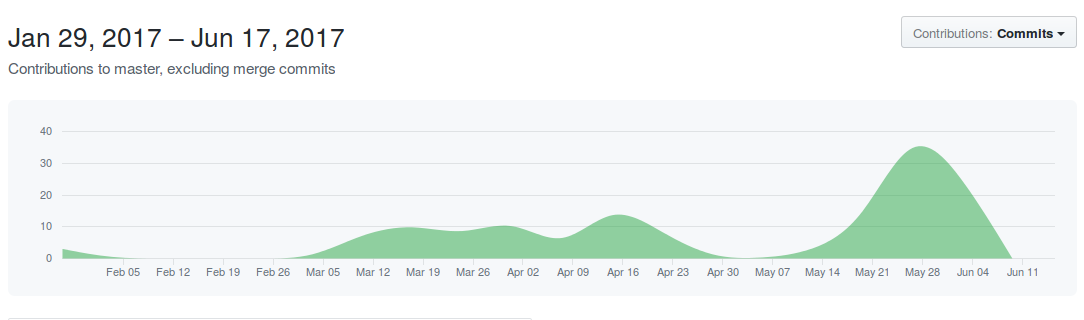
\includegraphics[scale=0.375]{Figures/commits_android.png}
\caption{Contribucions en el codi de l'aplicació}
\end{figure}
\begin{figure}[H]
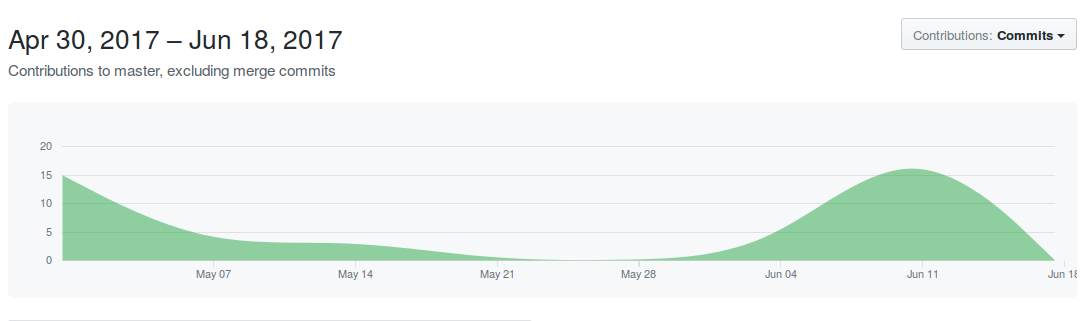
\includegraphics[scale=0.375]{Figures/commits_reports.png}
\caption{Contribucions en la memòria}
\end{figure}